\documentclass{article}

% --------------------------------------------------------------------
% Packages
% --------------------------------------------------------------------
\usepackage[utf8]{vietnam}
\usepackage{xcolor}
\usepackage{graphicx}
\usepackage{courier}
\usepackage[a4paper, pdftex, margin=1.5cm]{geometry}
\usepackage{setspace}
\usepackage{indentfirst}
\usepackage{tabularx}
\usepackage{amsmath}
\usepackage{tocloft}
\usepackage{hyperref}
\usepackage{sectsty}
\usepackage{listings}
\usepackage{enumerate}
\usepackage[shortlabels]{enumitem}
\usepackage{float}
\usepackage{algorithm} 
\usepackage{algpseudocode}
\usepackage{amssymb}
\graphicspath{ {./images/} }
\usepackage[utf8]{inputenc}
\usepackage{xcolor}
\usepackage{graphicx}
\usepackage{mathptmx} %font: Times
\usepackage{courier}
\usepackage[a4paper, pdftex, margin=1.5cm]{geometry}
\usepackage{setspace}
\usepackage{indentfirst}
\usepackage{tabularx}
\usepackage{amsmath}
\usepackage{tocloft}
\usepackage{hyperref}
\usepackage{sectsty}
\usepackage{listings}
\usepackage{enumerate}
\usepackage[shortlabels]{enumitem}
\usepackage{float}
% --------------------------------------------------------------------
% Definitions
% --------------------------------------------------------------------
\newcommand{\HRule}[1]{\rule{\linewidth}{#1}} 	% Horizontal rule

\makeatletter							% Title
\def\printtitle{%						
    {\centering \@title\par}}
\makeatother									

\makeatletter							% Author
\def\printauthor{%					
    {\centering \large \@author}}				
\makeatother							
\definecolor{LightYellow}{HTML}{ffffed}
\definecolor{LightBlue}{HTML}{326FC6}
\definecolor{LightBlue2}{HTML}{376BB4}
\definecolor{codegreen}{rgb}{0,0.6,0}
\definecolor{codegray}{rgb}{0.5,0.5,0.5}
\definecolor{codepurple}{rgb}{0.58,0,0.82}
\definecolor{backcolour}{rgb}{0.95,0.95,0.92}

\lstdefinestyle{mystyle}{
    backgroundcolor=\color{backcolour},   
    commentstyle=\color{codegreen},
    keywordstyle=\color{magenta},
    numberstyle=\tiny\color{codegray},
    stringstyle=\color{codepurple},
    basicstyle=\ttfamily\footnotesize,
    breakatwhitespace=false,         
    breaklines=true,                 
    captionpos=b,                    
    keepspaces=true,                 
    numbers=left,                    
    numbersep=5pt,                  
    showspaces=false,                
    showstringspaces=false,
    showtabs=false,                  
    tabsize=2
}
\begin{document}

\section{Giới thiệu bài toán Knapsack}
Bài toán knapsack là một bài toán tối ưu tổ hợp, input là một tập hợp các túi chứa vật (có 2 chỉ số weight và value). Output của bài toán là số túi sao cho cân nặng nhỏ hơn hoặc bằng cân nặng cho phép và giá trị là lớn nhất.Bài toán cái túi đã được nghiên cứu trong hơn một thế kỷ, với các công trình đầu tiên có niên đại từ năm 1897. Tên gọi "bài toán knapsack" có từ những công trình đầu tiên của nhà toán học Tobias Dantzig (1884–1956), và đề cập đến vấn đề phổ biến là đóng gói những vật phẩm hữu ích hoặc có giá trị nhất mà không làm quá tải hành lý.
\section{Thuật toán tiến hóa để giải bài toán knapsack}
Với bài toán knapsack,ta sẽ khởi tạo các tham số ban đầu của bài toán như sau
\begin{itemize}
    \item Initial Population: số cá thể ban đầu của bài toán
    \item Fitness Function: hàm số được chọn để ước lượng giá trị của cá thể
    \item Selection: lựa chọn cá thể để đột biến hoặc lai
    \item Crossover: tỉ lệ lai(thường rất cao để có thể đảm bảo có cá thể  đời sau có chất lượng tốt sinh ra
    \item Multation: tỉ lệ đột biến(thấp để đảm lời giải mới tìm được ít bị ảnh hưởng)
\end{itemize}
Với bài toán Knapsack có số lượng đồ vật là n:
\begin{itemize}
    \item Đầu tiên, ta sẽ khởi tạo kích thước quần thể(là số lời giải)
    \item Lựa chọn hàm số phù hợp cho bài toán Knapsack sao cho giá trị là lớn nhất với trọng lượng ở mức cho phép
    \item Lựa chọn các cá thể tốt nhất để tiến hành crossover
    \item lựa chọn crossover dựa trên one-point crossover
    \item với multation ta sẽ sử dụng kĩ thuật lật bit(bit đã được đột biến là 1,ngược lại là 0) 
\end{itemize}
Vì vậy các tham số bài toán được lựa chọn như sau
\begin{center}
        POPULATION SIZE $ \in$ (50,100,200,300)\\
        CROSSOVER $= 0.9$ \\
        MUTATION $= 0.1$   \\
        MAX GENERATIONS $= 50$
    \end{center}
Bằng viện phân tích thực nghiệm với thời gian giới hạn là 2 phút,ta có kết quả của các thuật toán tiến hóa như sau (chọn 3 loại đại diện group 0,6,12) và thay đổi POPULATIONSIZE (việc thay đổi tỉ lệ đột biến cao hơn sẽ làm cho lời giải mang tính ngẫu nhiên hơn(việc có kết quả tốt hay xấu phụ thuộc vào việc phần tử đột biến theo chiều hướng xấu hay tốt(ta không thể khống chế điều này)).Vì vậy ta chỉ cần giữ mức đột biến đủ nhỏ để chất lượng lời giải được đảm bảo sẽ tốt hơn.
\begin{enumerate}
    \item Với POPULATION SIZE=50:
\begin{center}
    \centering
    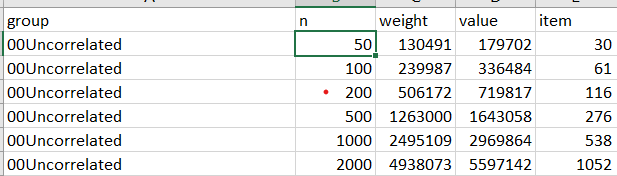
\includegraphics[width=15cm]{image/report1.png}
    \\
    \caption{ Result table for Uncorrelated group}
\end{center}
\begin{center}
    \centering
    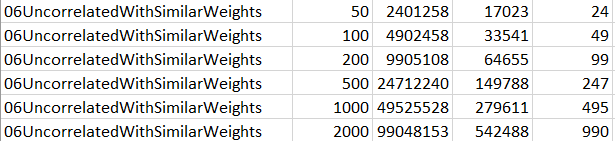
\includegraphics[width=15cm]{image/report2.png}
    \\
    \caption{ Result table for UncorrelatedWithSimilarWeights group}
\end{center}
\begin{center}
    \centering
    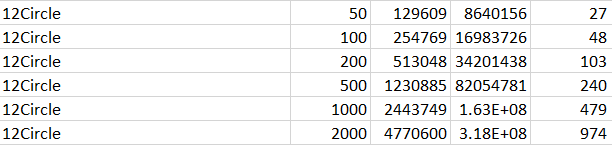
\includegraphics[width=15cm]{image/report3.png}
    \\
    \caption{ Result table for Circle group}
\end{center}
    \item Với POPULATION SIZE=100:
\begin{center}
    \centering
    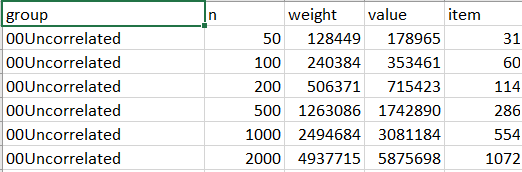
\includegraphics[width=15cm]{image/report4.png}
    \\
    \caption{ Result table for Uncorrelated group}
\end{center}
\begin{center}
    \centering
    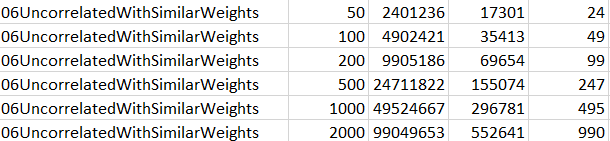
\includegraphics[width=15cm]{image/report5.png}
    \\
    \caption{ Result table for UncorrelatedWithSimilarWeights group}
\end{center}
\begin{center}
    \centering
    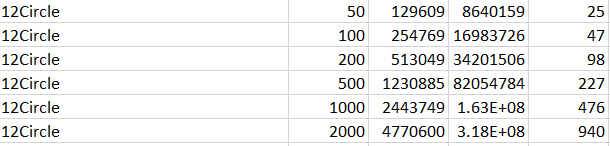
\includegraphics[width=15cm]{image/report6.png}
    \\
    \caption{ Result table for Circle group}
\end{center}
    \item Với POPULATION SIZE=200:
\begin{center}
    \centering
    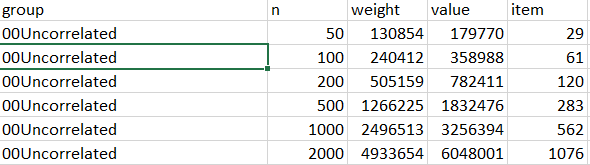
\includegraphics[width=15cm]{image/report7.png}
    \\
    \caption{ Result table for Uncorrelated group}
\end{center}
\begin{center}
    \centering
    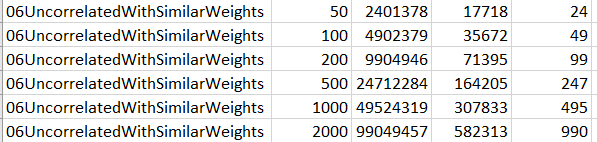
\includegraphics[width=15cm]{image/report8.png}
    \\\caption{ Result table for Uncorrelated group}
\end{center}
\begin{center}
    \centering
    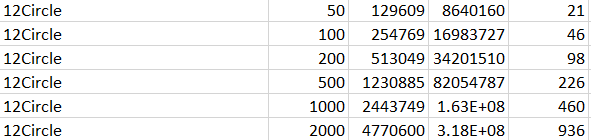
\includegraphics[width=15cm]{image/report9.png}
    \\\caption{ Result table for Uncorrelated group}
\end{center}
    \item Với POPULATION SIZE=300:
\begin{center}
    \centering
    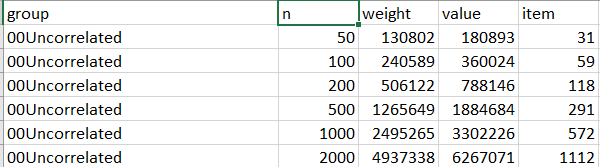
\includegraphics[width=15cm]{image/report10.png}
    \\\caption{ Result table for Uncorrelated group}
\end{center}
\begin{center}
    \centering
    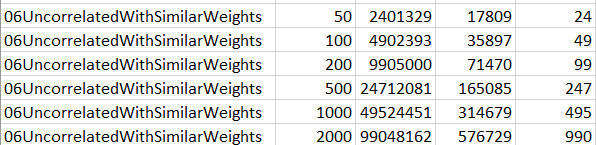
\includegraphics[width=15cm]{image/report11.png}
    \\\caption{ Result table for Uncorrelated group}
\end{center}
\begin{center}
    \centering
    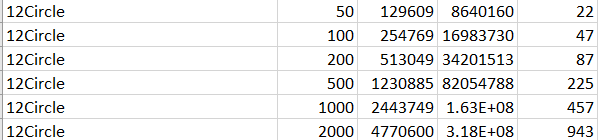
\includegraphics[width=15cm]{image/report12.png}
    \\\caption{ Result table for Uncorrelated group}
\end{center}
Ta sẽ trực quan hóa kết quả của các test group test case để dễ hình dung
 N
\begin{center}
    \centering
    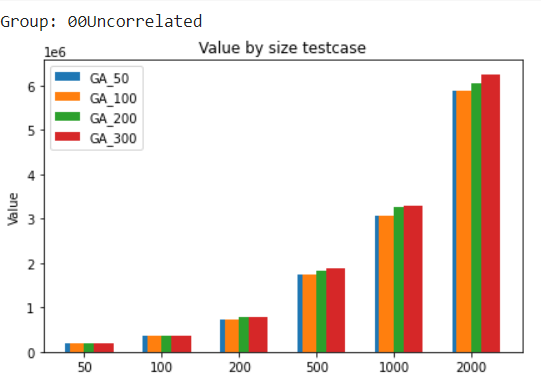
\includegraphics[width=15cm]{image/AI1.png}
\end{center}
\begin{center}
    \centering
    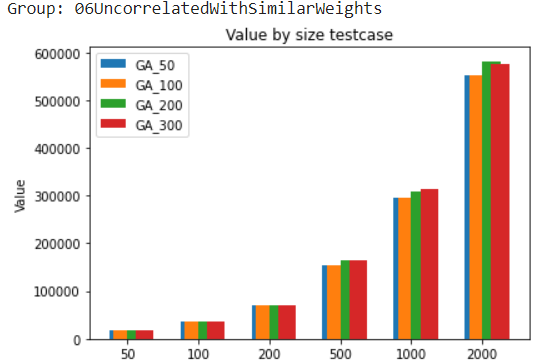
\includegraphics[width=15cm]{image/AI2.png}
\end{center}
\begin{center}
    \centering
    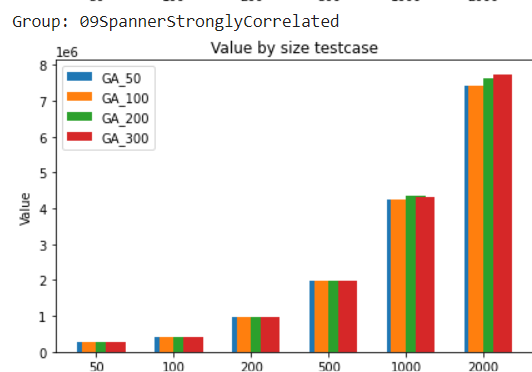
\includegraphics[width=15cm]{image/AI3.png}
\end{center}
\begin{center}
    \centering
    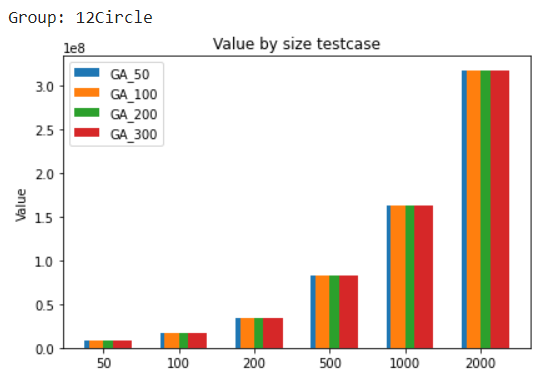
\includegraphics[width=15cm]{image/AI4.png}
\end{center}

\end{enumerate}\rar

Từ đó ta nhận thấy rằng với population càng cao thì lời giải sẽ có xu hướng càng tốt (có một số trường hợp không tốt bởi vì có sự đột biến(dù tỉ lệ rất nhỏ) bù lại thời gian thực thi sẽ chậm hơn
Vì vậy ta sẽ chọn lời giải POPULATION SIZE=300 để so sánh với việc sử dụng OR tools
\\
Ngoài ra vơi Max Generation=50 thì ở GA thời gian thực thi vẫn chưa phù hợp với thời gian giới hạn 2 phút.Vì thế ta sẽ set lại Max Generation là một số lớn để bài toán có thể chọn lọc ra lời giải tối ưu hơn
Chúng ta sẽ trực quan kết quả của các loại GA(2loại cuối là khi đã tune điều chỉnh max generation hợp lý ứng với thời gian giới hạn là 2 và 3 phút) để xem việc tăng maxgeneration hiệu quả không
\begin{center}
    \centering
    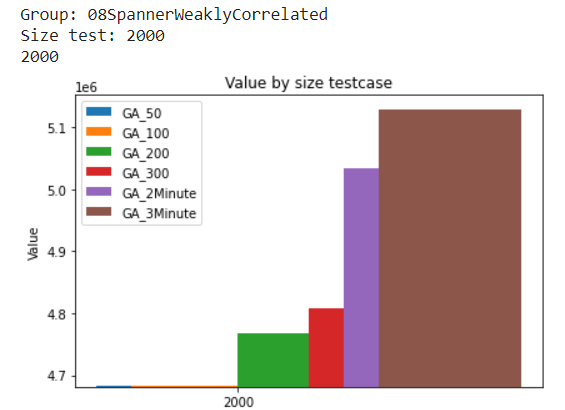
\includegraphics[width=15cm]{image/AI5.png}
\end{center}
\begin{center}
    \centering
    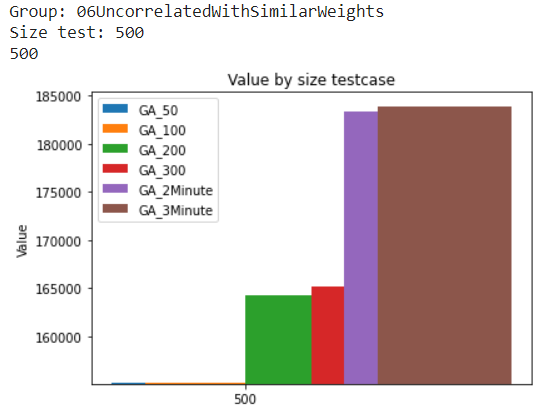
\includegraphics[width=15cm]{image/AI6.png}
\end{center}
\begin{center}
    \centering
    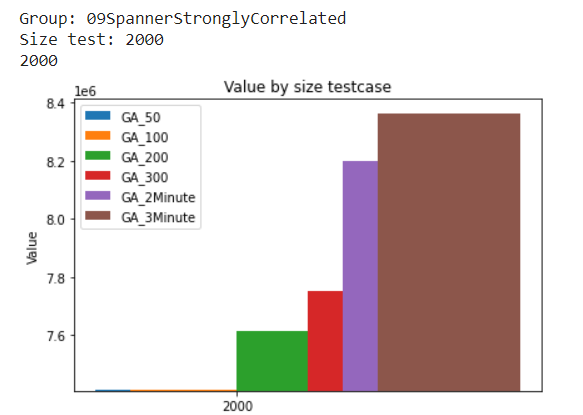
\includegraphics[width=15cm]{image/AI7.png}
\end{center}
\begin{center}
    \centering
    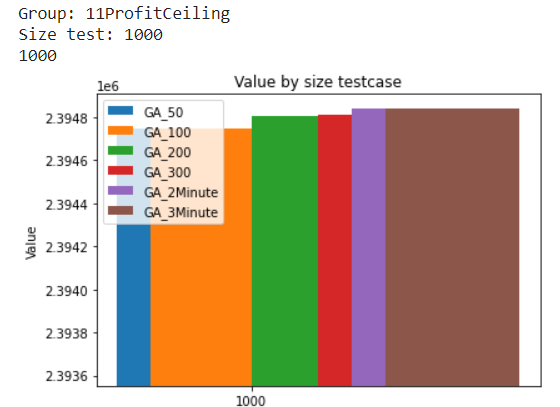
\includegraphics[width=15cm]{image/AI8.png}
\end{center}
\begin{center}
    \centering
    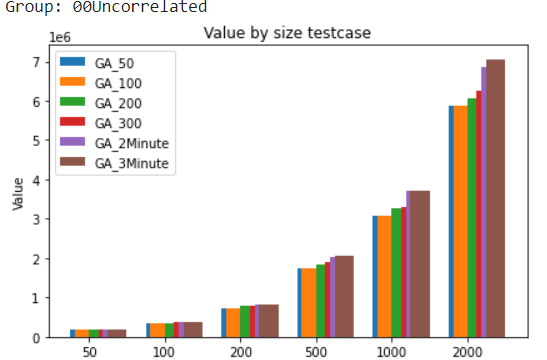
\includegraphics[width=15cm]{image/AI9.png}
\end{center}
\begin{center}
    \centering
    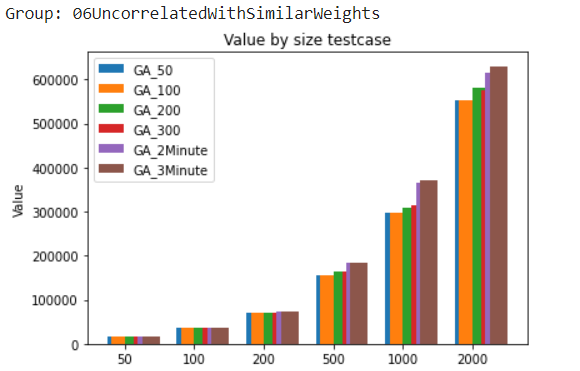
\includegraphics[width=15cm]{image/AI10.png}
\end{center}
\begin{center}
    \centering
    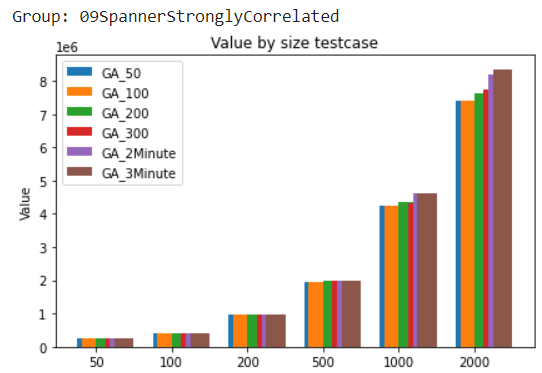
\includegraphics[width=15cm]{image/AI11.png}
\end{center}
\begin{center}
    \centering
    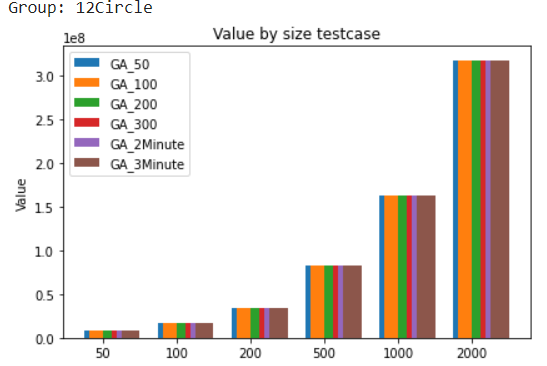
\includegraphics[width=15cm]{image/AI12.png}
\end{center}
Từ ta có thể thấy ở hầu hết các group thì kết quả của việc tối ưu maxgeneration là sẽ tốt hơn(việc để maxgeneration thấp sẽ khiến không tận dụng hết lượng populationsize lớn vì với số generation ít thì việc chọn lọc ra các lời giải tốt sẽ chưa có kết quả cao(kết quả ngày một cải thiện qua mỗi đời nhưng chưa cao) 



\section{Sử dụng OR Tool để giải Knapsack}
OR Tools là một công cụ mạnh mẽ được Google phát triển để giải quyết một số vấn đề  về các bài toá ntối ưu tổ hợp
Kết quả về độ chính xác của OR tools lầ rất mạnh mẽ(về độ chính xác thì không kém các cách giải truyền thống như QHĐ,quay lui nhưng thời gian thực thi tốt hơn
Ta sẽ xem kết quả bài toán ứng với 3 loại group test 4 loại group test đầu tiên(set timelimit là 2 phút)

\begin{center}
    \centering
    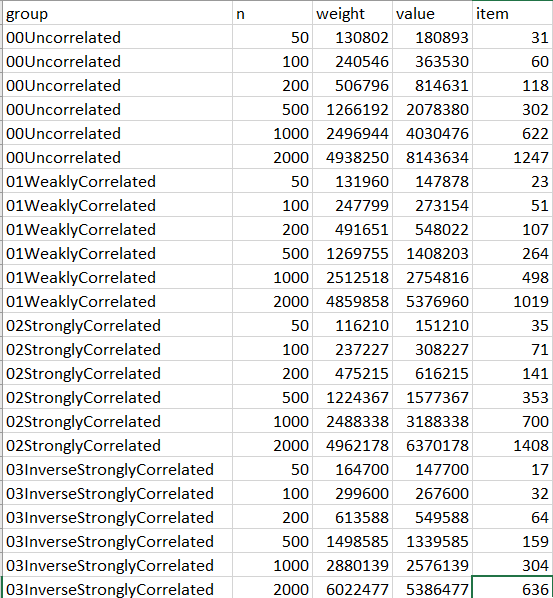
\includegraphics[width=15cm]{image/report13.png}
\end{center}
\section{So sánh kết quả của OR Tools và Genetic Algorithm}
Với cùng khoảng thời gian limit là 2 phút ta có kết quả như sau giữa lời giải Genetic(generation=50 và poplation=300) và OR :
\begin{center}
    \centering
    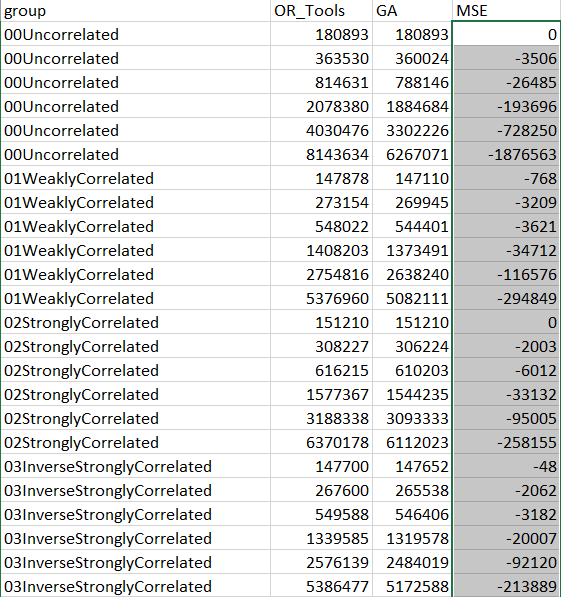
\includegraphics[width=15cm]{image/report14.png}
\end{center}
Từ đó ta thấy rằng với các test case nhỏ thì kết quả bài toán sẽ ít chêch lệch và khi số lượng vật ngày càng nhiều hơn thì sẽ có sự chênh lệch càng lớn(mặc dù thời gian chạy của các test OR chậm hơn)
\\
Ta sẽ xem kết quả trực quan sau khi tối ưu GA( so sánh GA300,GA2minute,GA3minute) và OR:
\begin{center}
    \centering
    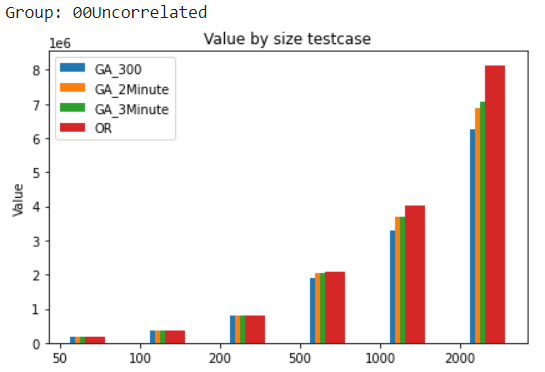
\includegraphics[width=15cm]{image/AI13.png}
\end{center}
\begin{center}
    \centering
    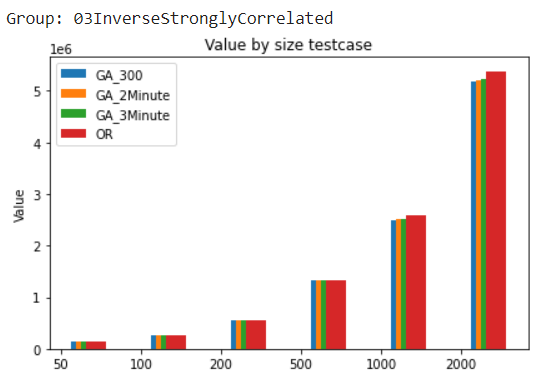
\includegraphics[width=15cm]{image/AI14.png}
\end{center}
\begin{center}
    \centering
    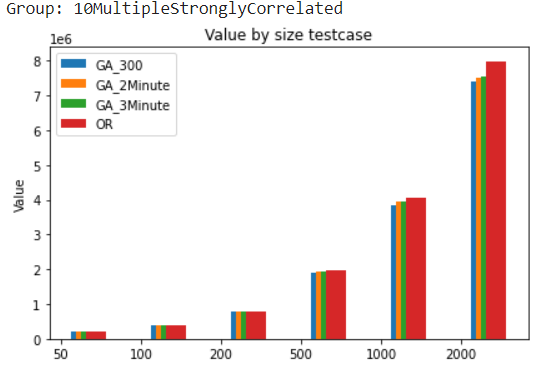
\includegraphics[width=15cm]{image/AI15.png}
\end{center}
\begin{center}
    \centering
    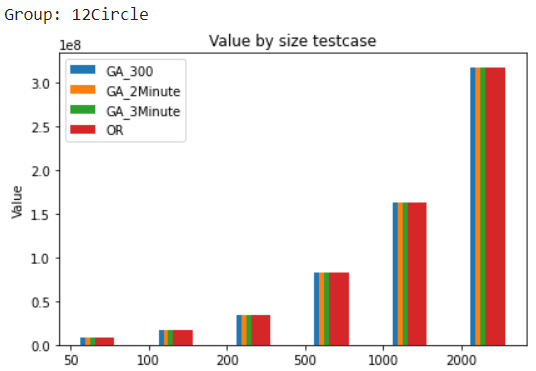
\includegraphics[width=15cm]{image/AI16.png}
\end{center}
\begin{center}
    \centering
    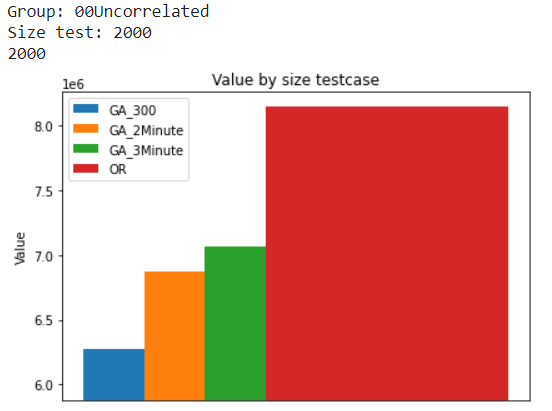
\includegraphics[width=15cm]{image/AI17.png}
\end{center}
\begin{center}
    \centering
    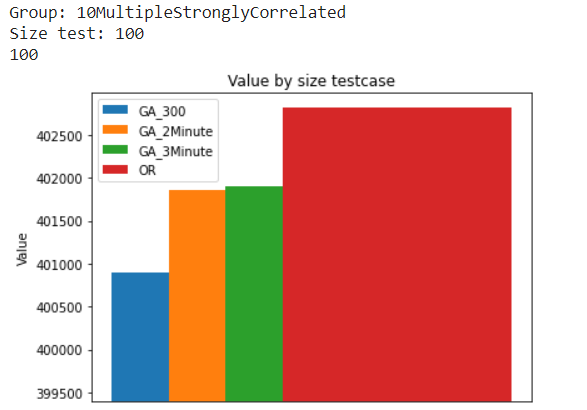
\includegraphics[width=15cm]{image/AI18.png}
\end{center}
\begin{center}
    \centering
    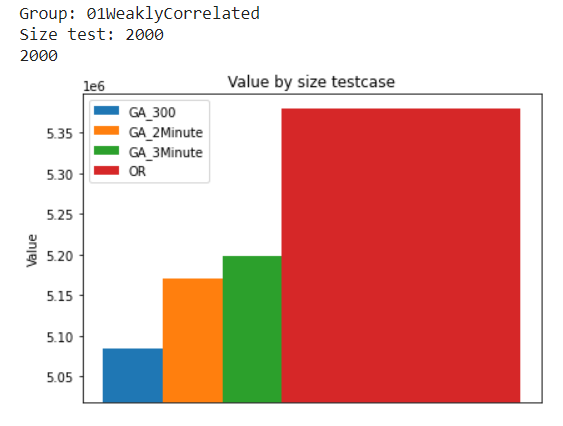
\includegraphics[width=15cm]{image/AI19.png}
\end{center}
Từ đó ta thấy rằng thuật toán OR hoạt động tốt hơn GA với population<=300, tuy nhiên nếu ta tăng population size càng cao thì liệu lời giải của GA có thể sẽ càng tốt (Kiểm chứng bằng thực nghiệm ).Vì vậy để cải thiện chất lượng lời giải ta có thể tăng giá trị populationsize để có thể có nhìu lời giải ban đầu nhằm dể dàng chọn lọc và cải thiện chất lượng hơn qua mỗi đời
\section{Tổng kết}
Kết quả thuật toán Genetic là chưa tối ưu vì số lượng generation vần còn ít và POPULATIONSIZE vẫn còn nhỏ,và nếu ta có thể tăng thời gian giới hạn và POPULATIONSIZE đủ lớn thì sẽ tìm ra được lời giải tối ưu,riêng trong tình huống thời gian và kích thước giới hạn như trên thì lời giải của OR tool sẽ tốt hơn một chút so với Genetic. Tuy vậy việc tối ưu population size đã nói ở trên vẫn có một vấn đề rằng liệu với một mức populatiosize nào đó thì chất lượng lời giải có cải thiện nữa không. Cần phải thực nghiệm thêm nhiều lần để đưa ra câu trả lời chính xác cho vấn đề này

\end{document}
